\documentclass[a4paper,12pt]{scrreprt}
    %% Used for changing geometry of the page
    %% Cover page text cannot overlay cover sketching/style
    %% https://ctan.org/pkg/geometry?lang=en
\usepackage{geometry}
    %% Changes language of some packages protocols
    %% e.g., when captioning images: Figure 1. -> Figura 1.
    %% https://ctan.org/pkg/babel?lang=en
\usepackage[portuguese]{babel}
    %% Used for special fonts
    %% Cannot be compiled with pdflatex
    %% https://ctan.org/pkg/fontspec?lang=en
\usepackage{fontspec}
    %% Arial FONT
    \setmainfont{Arial}

    %% More colors and color options
    %% https://ctan.org/pkg/xcolor?lang=en
    %% https://ctan.org/pkg/colortbl?lang=en
\usepackage{xcolor,colortbl}
    %% More tabular options, like dashed/dotted lines
    %% https://ctan.org/pkg/arydshln?lang=en
\usepackage{arydshln}
    %% List of acronyms
    %% https://ctan.org/pkg/nomencl?lang=en
\usepackage[intoc]{nomencl}
    %% Must be called to init nomencl environment
    \makenomenclature
    %% More images options/settings
    %% https://ctan.org/pkg/graphicx?lang=en
\usepackage{graphics}
    %% Defining subdirectories to image path enviornment
    %% \graphicspath{{sub1}{sub2}...{subN}}
    \graphicspath{{images}}

    %% used to handle cross-referencing commands in LaTeX to produce hypertext links in the document
    %% https://ctan.org/pkg/hyperref?lang=en
\usepackage{hyperref}
    %% math environments
    %% https://ctan.org/pkg/amsmath?lang=en

    %% settings
    \hypersetup{
        colorlinks,
        citecolor=black,
        filecolor=black,
        linkcolor=black,
        urlcolor=black
    }

\usepackage{amsmath}
    %% Defining backgrouns, used to make the cover
    %% https://ctan.org/pkg/background?lang=en
\usepackage[some]{background}
    %% Used to make drawings or complex graphics
    %% http://pgf.sourceforge.net/pgf_CVS.pdf
\usepackage{tikz}
    %% Tikz library to point operations ((x1,y1) + (x2,y2))
    \usetikzlibrary{calc}

%% Defining sfdefault font and default font for document
\renewcommand{\familydefault}{\sfdefault}

%==========================================================================
% DOCUMENT
%==========================================================================

\begin{document}

\pagenumbering{gobble}

%% Costume made cover
%% From there you can use \makecover command to build the cover
%% Blue cover color
\definecolor{titlepagecolor}{RGB}{208,112,68}

%==========================================================================
% COLORED BAR ON THE LEFT SIDE
%==========================================================================

\backgroundsetup{
    scale=1,
    angle=0,
    opacity=1,
    contents={
        \begin{tikzpicture}[remember picture,overlay]
            \path [fill=titlepagecolor] (-10.5,-15) rectangle ++ (5,30);
            \node[color=white] at (-7,-12) {\bfseries {\fontsize{120}{60} \textsf{P}}};
            \node[color=titlepagecolor] at (-4,-12) {\bfseries {\fontsize{120}{60} \textsf{O}}};
            \node[color=titlepagecolor] at (-1,-12) {\bfseries {\fontsize{120}{60} \textsf{O}}};
        \end{tikzpicture}
    }
}

%==========================================================================
% TITLE PAGE INFO
%==========================================================================

%% Changes values in this field to show information in the cover and back cover about your team/project

%% TITLE
\title{TODO - title}

%% AUTHORS
\author{
    Flávia Alexandra Silva Araújo (A96587) \\
  \quad
    Miguel Torres Carvalho (A95485)
}

%% Date

\date{\today}

%% Course
\newcommand{\Course}{Licenciatura em Engenharia Informática}

%% Department
\newcommand{\Department}{Escola de Engenharia}

%% UniName
\newcommand{\UniName}{Universidade do Minho}

%% UniPic
\newcommand{\UniPic}{
\includegraphics[scale=0.5]{images/eeum.png}}

%% University
\newcommand{\University}{
    \begin{flushleft}
        \UniPic
    \end{flushleft}
    \textcolor{gray}{\small\textbf{\textsf{\UniName}}}\par
    \textcolor{gray!80!white}{\small{\textsf{\Department}}}\par
    \textcolor{gray!70!white}{\small{\textsf{\Course}}}
}

%% UC
\newcommand{\UC}{
    \begin{flushleft}
        \par\textcolor{titlepagecolor}{  \LARGE\textbf{\textsf{Unidade Curricular de \\ Programação Orientada a Objetos}}}
    \end{flushleft}
}

%% School Year
\newcommand{\SchoolYear}{
    \small{\textsf{Ano Letivo de 2023/2024}}}


%% Define new command to show title, author and date
\makeatletter
\let\Title\@title
\let\Author\@author
\let\Date\@date
\makeatother

%==========================================================================
% CLASSIFICATION SECTION
%==========================================================================

%% School Year
\newcommand{\ReceptionDate}{}
%% Responsible
\newcommand{\Responsible}{}
%% Evaluation
\newcommand{\Evaluation}{}
%% Observations
\newcommand{\Observations}{}

%% MAKETEMPLATE
\newcommand{\makecover}{

%==========================================================================
% BEGIN COVER PAGE
%==========================================================================

%% Removes page number on footer
\thispagestyle{empty}

%% No indentation
\setlength{\parindent}{0em}

%% Put Background defined on \backgroundsetup, in this page
\BgThispage

%% Changing geometry to prevent overlay with text
%% At the end of back cover, geometry is default with \restoregeometry
\newgeometry{top=5cm,left=6cm,right=3cm,bottom=2cm}

%% builds university info defined previously
\University
\vspace{1cm}
%% builds curricular unity info defined previously
\UC
%% builds school year info defined previously
\SchoolYear

\vspace*{5cm}
%% bigger space (i think its the default one) between paragraphs
\setlength{\parskip}{1em}

%% builds title info defined previously
\par\textbf{\textsf{\huge\Title}}
\vspace{1cm}
%% builds author(s) info defined previously
\par\Author

\vspace{0.5cm}

%% builds date info defined previously
\par\Date
\restoregeometry
\pagebreak

%==========================================================================
% END COVER PAGE
%==========================================================================

%==========================================================================
% BEGIN BACK COVER PAGE
%==========================================================================

%% Removes page number on footer
\thispagestyle{empty}

\textbf{Equipa de Trabalho:}

% \begin{center}

\includegraphics[scale=0.5]{images/flavia.png} \\
\textbf{Flávia Alexandra Silva Araújo (A96587)} \\ \\

\includegraphics[scale=0.5]{images/miguel.png} \\
\textbf{Miguel Torres Carvalho (A95485)}
% \end{center}

\pagebreak
%==========================================================================
% END BACK COVER PAGE
%==========================================================================
}


% builds the cover
\makecover

%% smaller footer and header size
\newgeometry{top=3cm,left=3cm,right=3cm,bottom=4cm}
\savegeometry{default}

%==========================================================================
% BEGIN ABSTRACT PAGE
%==========================================================================

% Abstract name: \Large font size, flushed left and paragraph skip before abstract content
\renewenvironment{abstract}
 {\par\noindent\textbf{\Large\abstractname}\par\bigskip}
 {}

\begin{flushleft}
\begin{abstract}
    No âmbito da Unidade Curricular Programação Orientada a Objetos, foi-nos proposto o
    desenvolvimento de uma aplicação de gestão de atividades físicas, à qual desginamos de \textit{Activity Planner}.

    A aplicação desenvolvida permite a gestão de utilizadores, atividades, planos de treino, simulação de atividades e
    visualização de estatísticas. A aplicação foi desenvolvida em \textit{Java}, utilizando o paradigma de programação
    orientada a objetos aprendido nas aulas.

    Neste relatório, é apresentada a arquitetura de classes da aplicação, bem
    como as funcionalidades implementadas nesta e a forma como as mesmas foram desenvolvidas.
\end{abstract}
\end{flushleft}

%==========================================================================
% END ABSTRACT PAGE
%==========================================================================

%==========================================================================
% BEGIN INDEXES PAGES
%==========================================================================

%% Changes table of content name
%% Portuguese babel default : "Conteúdo"
%% Personally I prefer "índice"
\renewcommand{\contentsname}{Índice}
% \renewcommand{\listfigurename}{Índice de Figuras}
% \renewcommand{\listtablename}{Índice de Tabelas}

\tableofcontents
\pagebreak
\listoffigures
\pagebreak
% \listoftables
% \pagebreak

%==========================================================================
% END INDEXES PAGES
%==========================================================================

%==========================================================================
% BEGIN ARQUITETURA DE CLASSES
%==========================================================================

%% Starting page numbering here
\pagenumbering{arabic}

\chapter{Arquitetura de Classes}
\section{Diagrama de Classes}
    \begin{minipage}{\textwidth}
        \centering
        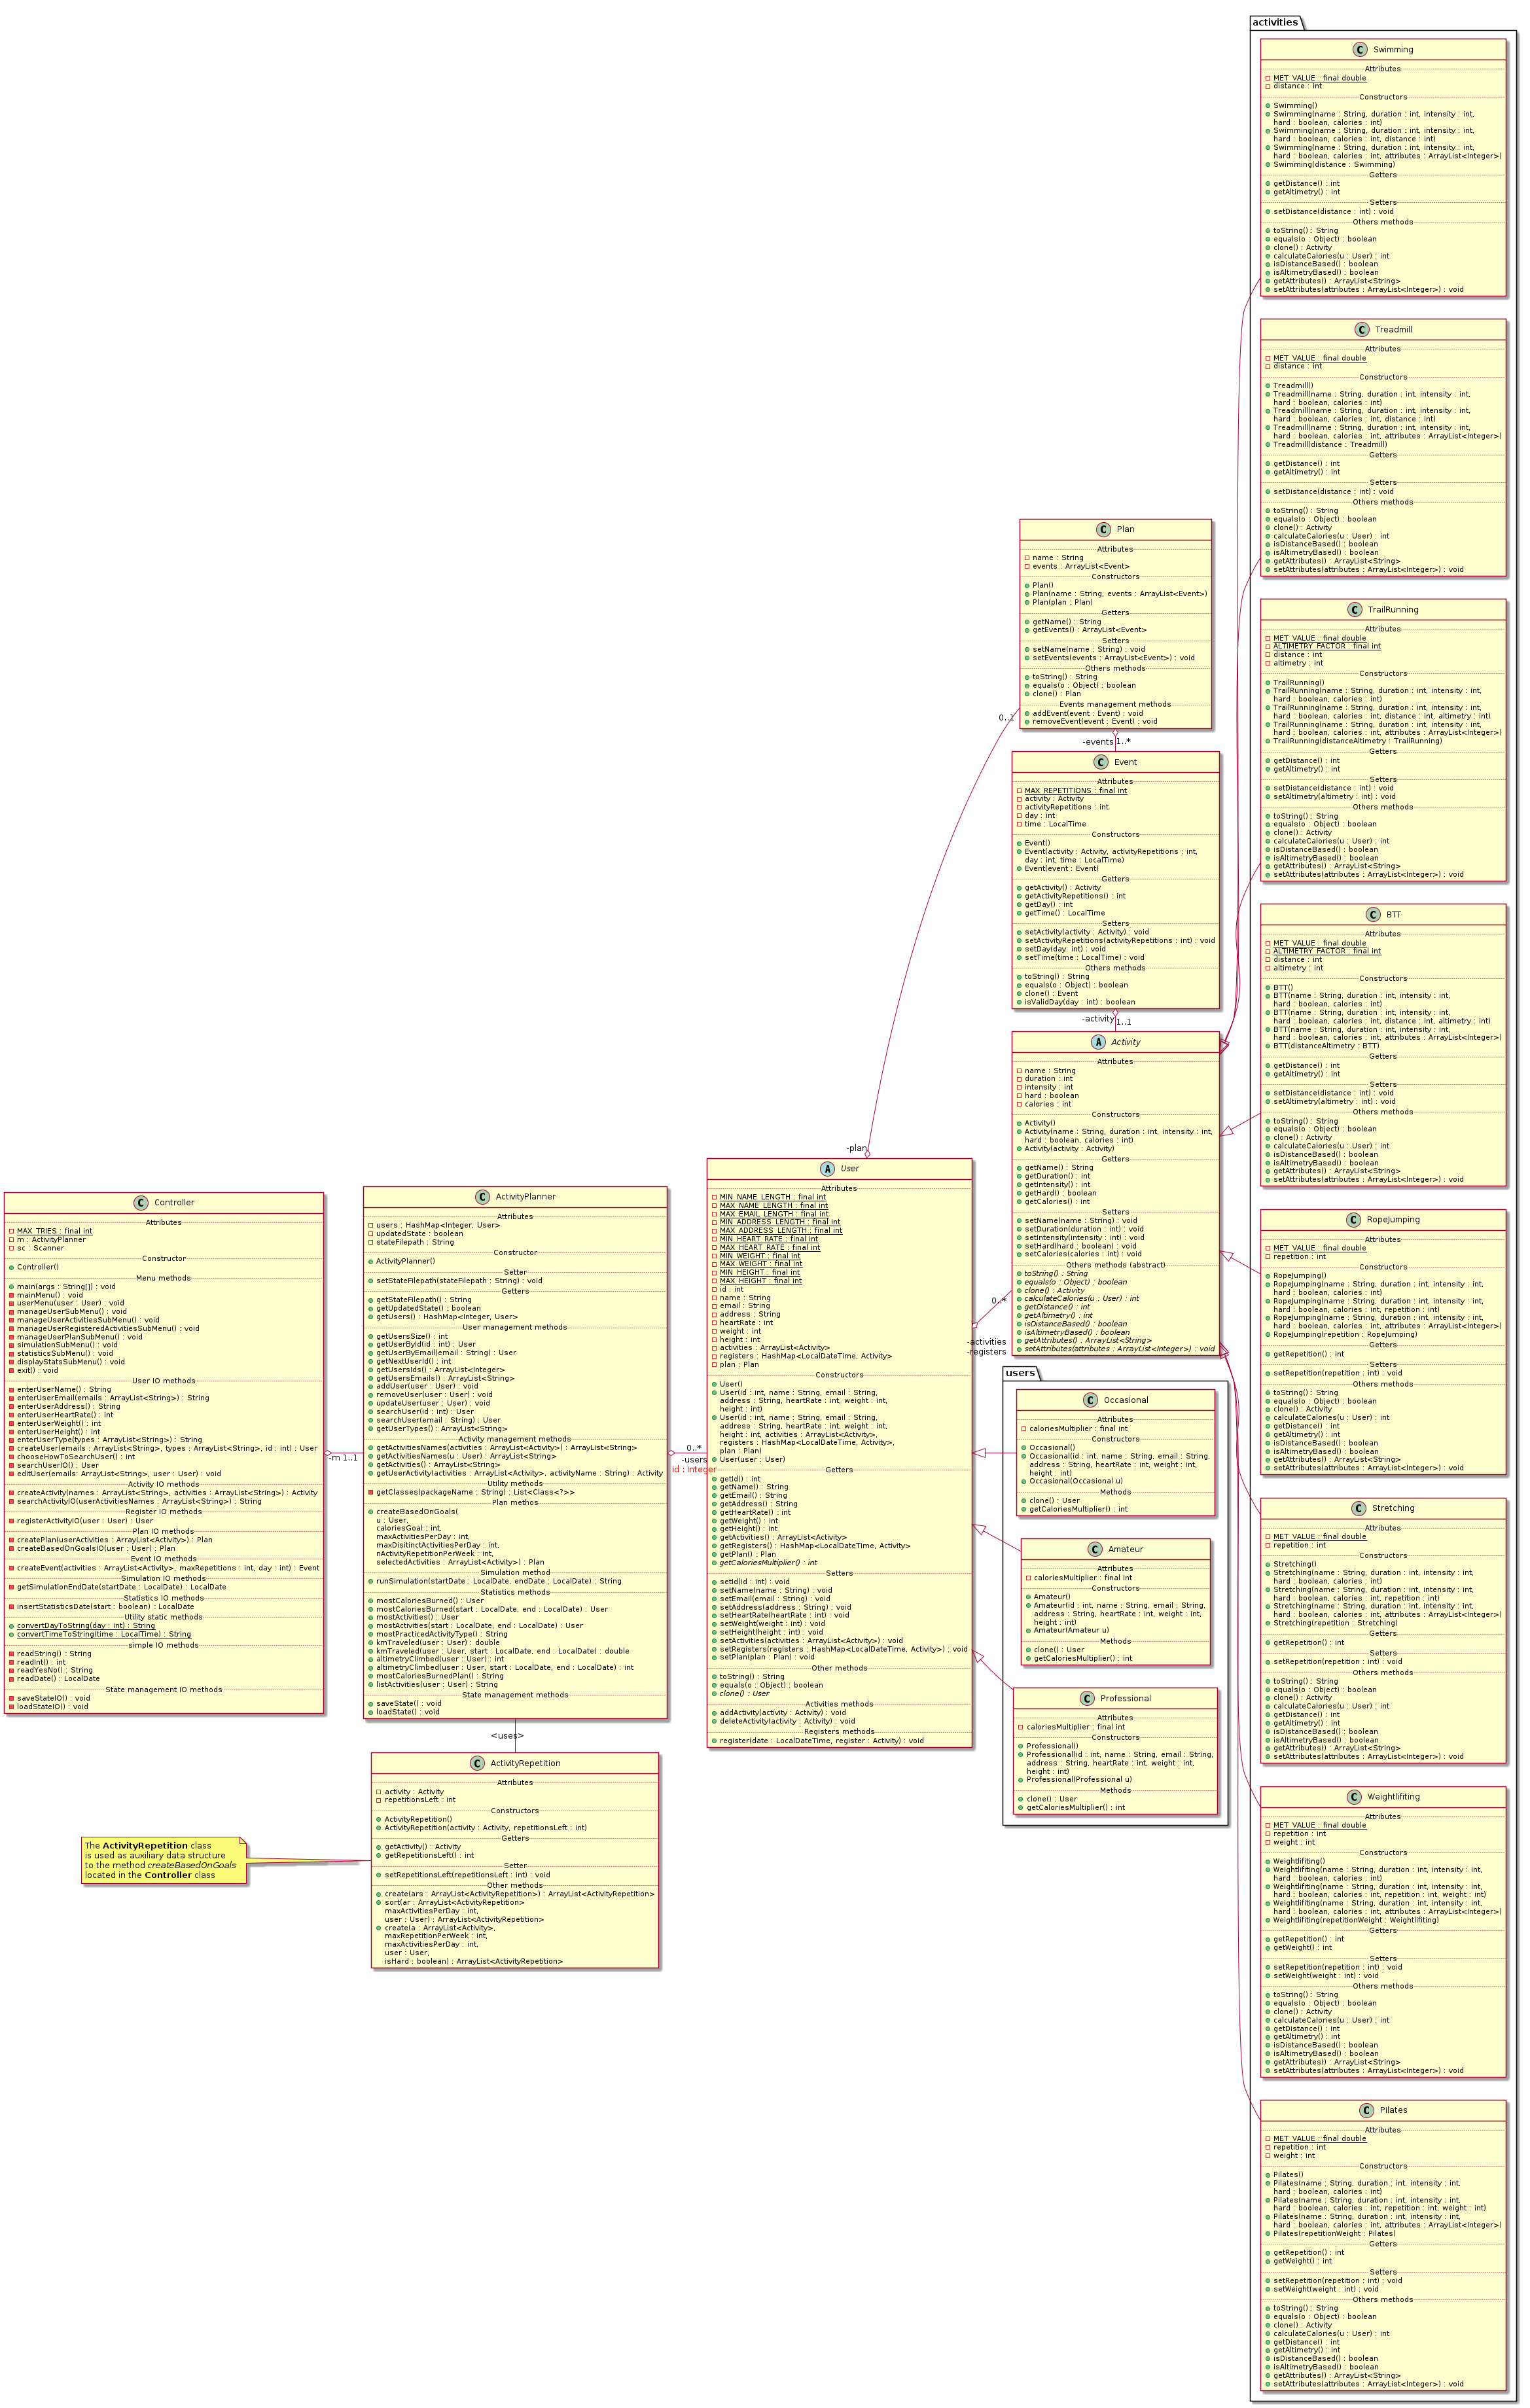
\includegraphics[width=\textwidth]{images/diagram.png}
        \captionof{figure}{Diagrama de Classes}
        \label{fig:diagrama-classes}
    \end{minipage}

\section{Classe \textit{ActivityPlanner}}
    A classe \textit{ActivityPlanner} funciona como o modelo e \textit{facade} da aplicação,
    sendo responsável por guardar e carregar o estado da aplicação,
    bem como por fornecer métodos para a manipulação e acesso deste estado.

    Por conseguinte, a \textit{ActivityPlanner} é constituída pelos seguintes atributos:

    \begin{itemize}
        \item \textit{\textbf{users : HashMap<Integer, User>}} - Lista de utilizadores carregados;
        \item \textit{\textbf{updatedState : boolean}} - Indica se o estado da aplicação foi alterado;
        \item \textit{\textbf{defaultStateFilepath : String}} - Caminho para o ficheiro binário que contém o estado da aplicação.
    \end{itemize}

    Providencia métodos para a gestão de utilizadores, acesso ao nome de atividades, simulação de atividades e cálculo de estatísticas,
    assim como para a salvaguarda do estado da aplicação e métodos que retornam a lista das subclasses de \textit{User} e \textit{Activity},
    utilizados para a listagem de utilizadores e atividades oferecidas pela aplicação, ao criar um novo utilizador ou atividade iterativamente,
    na classe \textit{Controller}.

\clearpage

\newgeometry{top=2.5cm,left=3cm,right=3cm,bottom=3cm}
\section{Classe \textit{Controller}}
    A classe \textit{Controller} é a classe responsável pela execução do programa -
    faz o \textit{parsing} dos argumentos da linha de comandos,
    carrega e salva o estado da aplicação através da classe \textit{ActivityPlanner},
    e executa o menu principal ou da perspetiva de um utilizador, dependendo dos argumentos passados.

    É nesta classe que ocorrem as interações com o utilizador, através de menus interativos,
    e a execução das funcionalidades da aplicação.

    Foram desenvolvidos os seguintes menus interativos, com os respetivos submenus e opções:
    \begin{itemize}
        \item Menu principal da aplicação:
        \begin{itemize}
            \item Adicionar, editar, remover e visualizar utilizadores;
            \item Adicionar, remover e visualizar atividades de interesse;
            \item Registar e visualizar atividades completas;
            \item Adicionar, remover e visualizar planos de treino;
            \item Simular atividades;
            \item Visualizar estatísticas;
            \item Carregar e guardar o estado da aplicação;
            \item Sair da aplicação.
        \end{itemize}
        \item Menu com a perspetiva de um utilizador:
        \begin{itemize}
            \item Editar o perfil do utilizador;
            \item Adicionar e remover atividades de interesse;
            \item Registar e visualizar atividades completas;
            \item Adicionar, remover e visualizar planos de treino;
            \item Visualizar estatísticas;
            \item Carregar e guardar o estado da aplicação;
            \item Sair da aplicação.
        \end{itemize}
    \end{itemize}

    A classe \textit{Controller} funciona como uma \textit{interface} entre o utilizador e a aplicação,
    sendo responsável por chamar os métodos da classe \textit{ActivityPlanner} e por apresentar os resultados.

    No sistema MVC esta classe representa o \textit{controller} assim como o \textit{view},
    uma vez que é responsável por apresentar os menus interativos,
    fazendo as respetivas execuções através dos métodos da classe \textit{ActivityPlanner}.

\clearpage
\section{Classe \textit{User}}
    A superclasse \textit{User} representa um utilizador da aplicação, sendo constituída pelos seguintes atributos:

    \begin{itemize}
        \item \textit{\textbf{id : int}} - Identificador único do utilizador;
        \item \textit{\textbf{name : String}} - Nome completo do utilizador;
        \item \textit{\textbf{email : String}} - Endereço de correio eletrónico do utilizador, sendo este único em relação a todos os utilizadores da aplicação;
        \item \textit{\textbf{address : String}} - Morada do utilizador;
        \item \textit{\textbf{heartRate : int}} - Frequência cardíaca em repouso do utilizador, em batimentos por minuto;
        \item \textit{\textbf{weight : int}} - Peso do utilizador, em kilogramas;
        \item \textit{\textbf{height : int}} - Altura do utilizador, em centímetros;
        \item \textit{\textbf{activities : ArrayList<Activity>}} - Conjunto de atividades de interesse de um utilizador, utlizada para a simplificação de um registo da atividade praticada ou da criação de um plano de treino;
        \item \textit{\textbf{registers : HashMap<LocalDateTime, Activity>}} - Conjunto de actividades praticadas por um utilizador, com a respetiva data e hora de prática, atividade praticada e consumo calórico;
        \item \textit{\textbf{plan : Plan}} - Plano de treino semanal de um utilizador.
    \end{itemize}

    Os atributos \textit{weight}, \textit{height} e \textit{heartRate} são utilizados para o cálculo do consumo calórico de uma atividade,
    sendo estes parâmetros mutáveis, uma vez que podem ser alterados ao longo do tempo.

    Para além dos vários construtores, dos métodos tradicionais de acesso e modificação dos atributos (\textit{getters} e \textit{setters}), métodos para a cópia profunda dos objetos desta classe, conversão para \textit{String} e igualdade entre objetos desta classe, foram implementados métodos para a adição/remoção de uma atividade de interesse, bem como métodos para o registo de uma atividade por parte de um utlizador.

    A classe \textit{User} foi desenvolvida de forma a permitir a extensão desta, através da implementação de novos tipos de utilizadores.
    Assim, foi definida uma hierarquia de classes, onde a classe \textit{User} é a superclasse e as suas subclasses são \textit{Occasional}, \textit{Amateur} e \textit{Professional}.

    A aplicação foi desenvolvida de forma a permitir a adição de novos tipos de utilizadores,
    através da criação de uma nova subclasse de \textit{User} com as características específicas deste tipo de utilizador,
    sem que fosse necessário alterar a classe \textit{User} e outras componentes da aplicação,
    garantindo, deste modo, a modularidade, manutenção e extensabilidade da superclasse \textit{User} e das suas subclasses.

\loadgeometry{default}
\clearpage
\section{Classe \textit{Activity}}
    A superclasse \textit{Activity} representa uma atividade física, sendo constituída pelos seguintes atributos:

    \begin{itemize}
        \item \textit{\textbf{name : String}} - Nome da atividade;
        \item \textit{\textbf{duration : int}} - Duração da atividade, em minutos;
        \item \textit{\textbf{intensity : int}} - Intensidade da atividade (um valor de 1 a 100 para representar um valor percentual);
        \item \textit{\textbf{hard : boolean}} - Indica, através de um valor booleano, se a atividade é considerada \textit{hard} pelo utilizador;
        \item \textit{\textbf{calories : int}} - Número de calorias queimadas durante a atividade. O registo deste atributo deve-se à mutação dos parâmetros do utilizador para o cálculo do consumo calórico, desde a frequência cardíaca, o peso, bem como a altura deste. Assim, este atributo foi utilizado de forma a garantir a salvaguarda do valor de calorias queimadas num registo de uma atividade.
    \end{itemize}

    A classe \textit{Activity}, assim como a classe \textit{User}, foi desenvolvida de forma a permitir a extensão desta,
    através da implementação de novos tipos de atividades, sem que fosse necessário alterar a classe \textit{Activity} e
    outras componentes da aplicação.

    As subclasses de \textit{Activity} contêm atributos específicos que caracterizam a atividade em questão,
    como por exemple, a distância percorrida, o número de repetições, o peso levantado, entre outros.

    Foram implementadas as seguintes subclasses de \textit{Activity}:
    \begin{itemize}
        \item \textit{\textbf{Swimming}} - Atividade de natação, compostas pelos atributos \textit{distance : int};
        \item \textit{\textbf{Treadmill}} - Atividade de corrida em passadeira, compostas pelos atributos \textit{distance : int};
        \item \textit{\textbf{TrailRunning}} - Atividade de corrida em trilhos, compostas pelos atributos \textit{distance : int} e \textit{altimetry : int};
        \item \textit{\textbf{BTT}} - Atividade de BTT, compostas pelos atributos \textit{distance : int} e \textit{altimetry : int};
        \item \textit{\textbf{RopeJumping}} - Atividade de saltar à corda, compostas pelos atributos \textit{repetitions : int};
        \item \textit{\textbf{Stretching}} - Atividade de alongamentos, compostas pelos atributos \textit{repetitions : int};
        \item \textit{\textbf{Weightlifting}} - Atividade de levantamento de pesos, compostas pelos atributos \textit{repetitions : int} e \textit{weight : int};
        \item \textit{\textbf{Pilates}} - Atividade de pilates, compostas pelos atributos \textit{repetitions : int} e \textit{weight : int};
    \end{itemize}

    Para cada uma destas subclasses é definido o atributo MET (\textit{Metabolic Equivalent of Task}) da atividade,
    que é utilizado para o cálculo do consumo calórico da atividade,
    este também definido como um método abstrato na superclasse \textit{Activity}.

    Nas subclasses de \textit{Activity} foram implementados métodos para obter e definir os atributos específicos da atividade,
    estes permitem a criação destas atividades de forma iterativa, através da classe \textit{Controller}.

    A classe \textit{Activity} foi desenvolvida tirando proveito do conceito de polimorfismo,
    permitindo a criação de atividades de forma genérica, através da superclasse \textit{Activity},
    e a sua manipulação de forma específica, através dos atributos únicos das respetivas subclasses.

\section{Classe \textit{Event}}
    A classe \textit{Event} representa um evento correspondente a um plano de treino, sendo constituída pelos seguintes atributos:

    \begin{itemize}
        \item \textit{\textbf{activity : Activity}} - Atividade praticada no evento;
        \item \textit{\textbf{activityRepetitions : int}} - Número de vezes que a atividade será praticada;
        \item \textit{\textbf{day : int}} - Dia da semana do evento, onde 1 corresponde a domingo e 7 a sábado;
        \item \textit{\textbf{time : LocalTime}} - Hora do evento.
    \end{itemize}

\section{Classe \textit{Plan}}
    A classe \textit{Plan} representa um plano de treino, por definição, semanal, que um utilizador pode criar, vizualizar e remover.

    Esta é composta pelos seguintes atributos:
    \begin{itemize}
        \item \textit{\textbf{name : String}} - Nome do plano de treino;
        \item \textit{\textbf{events : ArrayList<Event>}} - Lista de eventos que compõem o plano de treino.
    \end{itemize}

    As funcionalidades proporcionadas por esta classe, bem como a classe \textit{Event}, serão detalhadas no subcapítulo \textit{\nameref{sec:gestao-planos-treino}}.

\section{Classe \textit{ActivityRepetition}}
    A classe \textit{ActivityRepetition} é utlizada como um objeto auxiliar para a criação de um plano de treino baseado nos objetivos de um utilizador.

    O processo de geração de planos de treino baseados em objetivos será aprofundado no subcapítulo \textit{\nameref{sec:gestao-planos-treino}},
    a qual será detalhada a forma como esta classe é utilizada.

\section{Package \textit{exceptions}}
    Foi também criado um \textit{package} \textit{exceptions}, onde foram definidas as seguintes exceções:

    \begin{itemize}
        \item \textit{\textbf{ActivityIsRegisteredException}} - Exceção lançada quando uma atividade com o mesmo nome já foi registada;
        \item \textit{\textbf{ActivityNotFoundException}} - Exceção lançada quando uma atividade não é encontrada;
        \item \textit{\textbf{UserNotFoundException}} - Exceção lançada quando um utilizador não é encontrado;
        \item \textit{\textbf{StateNotSavedException}} - Exceção lançada quando o estado da aplicação não pode ser guardado;
        \item \textit{\textbf{StateNotLoadedException}} - Exceção lançada quando o estado da aplicação não pode ser carregado;
    \end{itemize}

    Estas exceções foram criadas de forma a garantir a robustez da aplicação,
    permitindo a deteção de situações de erro e a sua correta gestão.

%==========================================================================
% END ARQUITETURA DE CLASSES
%==========================================================================

%==========================================================================
% BEGIN DESCRIÇÃO DE FUNCIONALIDADES DA APLICAÇÃO
%==========================================================================

\chapter{Descrição de Funcionalidades da Aplicação}

\section{Gestão de Utilizadores}
    \label{sec:gestao-utlizadores}
    \subsection{Adicionar Utilizador}
    \textcolor{red}{TODO}
    \subsection{Editar Utilizador}
    \textcolor{red}{TODO}
    \subsection{Remover Utilizador}
    \textcolor{red}{TODO}
    \subsection{Visualizar Utilizadores}
    \textcolor{red}{TODO}

\section{Gestão de Atividades}
    \label{sec:gestao-atividades}
    \subsection{Adicionar Atividade}
    \textcolor{red}{TODO}
    \subsection{Remover Atividade}
    \textcolor{red}{TODO}
    \subsection{Visualizar Atividades}
    \textcolor{red}{TODO}

\section{Registo e Visualização de Atividades Completas}
    \label{sec:registo-atividades}
    \subsection{Registar Atividade}
    \textcolor{red}{TODO}
    \subsection{Visualizar Registos de Atividades}
    \textcolor{red}{TODO}

\section{Gestão de Planos de Treino}
    \label{sec:gestao-planos-treino}
    \subsection{Adicionar Plano de Treino Interativamente}
    \textcolor{red}{TODO}
    \subsection{Adicionar Plano de Treino Baseado em Objetivos}
    \textcolor{red}{TODO}
    \subsection{Remover Plano de Treino}
    \textcolor{red}{TODO}
    \subsection{Visualizar Planos de Treino}
    \textcolor{red}{TODO}

\section{Simulação}
    \label{sec:simulacao}
    \textcolor{red}{TODO}

\section{Estatísticas}
    \label{sec:estatisticas}
    \textcolor{red}{TODO}

\clearpage
\section{Salvaguarda do Estado da Aplicação}
    \label{sec:salvaguarda-estado}
Para garantir que o estado da aplicação é preservado entre execuções, esta
permite guardar e carregar o estado atual através de um ficheiro binário.
As opcões de guardar e carregar o estado do programa estão disponíveis no menu principal da aplicação. Adicionalmente o ficheiro binário pode ser carregado diretamente no início da execução do programa através da passagem da localização deste na linha de comandos.
Este ficheiro, por definição, é guardado na diretoria \textit{data} e tem o nome \textit{state.ser}, havendo a opção de carregar diferentes estados através da funcionalidade da linha de comandos supramencionada.

Para a implementação desta funcionalidade foram definidos dois métodos na classe \textit{Main}:
\begin{itemize}
    \item \textit{saveState} - Método que guarda o estado atual da aplicação num ficheiro binário, passado como argumento. Este método deteta se alguma mudança foi feita no estado do programa antes de a guardar, de forma evitar salvar o mesmo estado.
    \item \textit{loadState} - Método que carrega o estado da aplicação a partir de um ficheiro binário, passado como argumento.
\end{itemize}

Como os objetos da classe \textit{User} contêm referências para todos os objetos relevantes de serem guardados/carregados - lista de Atividades, conjunto de registos de atividades, Plano de treino semanal com os respetivos Eventos - foi necessário garantir que estes e a própria classe referente ao Utilizador implementassem a interface \textit{Serializable}, de forma a que fossem possíveis de ser guardados, e futuramente carregados, num ficheiro binário.

A aplicação também dispõe de uma capacidade inteligente de detetar mudanças no seu estado, através do atributo booleano \textit{updatedState} na classe \textit{Main}, o que permitiu a implementação das seguintes funcionalidades:

\begin{itemize}
    \item Notificar o utilizador de que o estado atual não foi guardado, caso este tente sair da aplicação, dando a opção de o guardar, caso o utilizador o deseje fazer.
    \item Notificar o utilizador que, ao carregar um novo estado, o estado atual será perdido, se houver alterações, dando a opção de retornar atrás se este não quiser perder o estado atual.
\end{itemize}

O valor do atributo \textit{updatedState} é incializado a \textit{false} no ínicio da execução do programa e é alterado para \textit{false} sempre que o estado da aplicação é guardado, no método \textit{saveState}, ou carregado, no método \textit{loadState}, referidos anteriormente.

Este valor booleano é alterado para \textit{true} sempre que o estado da aplicação é alterado, seja através da adição, edição ou remoção de um utilizador, de uma atualização de uma atividade de um utilizador, do registo de uma nova atividade ou da criação/remoção de um plano de treino para um utlizador em específico.

\section{Argumentos de Linha de Comandos}

%==========================================================================
% END DESCRIÇÃO DE FUNCIONALIDADES DA APLICAÇÃO
%==========================================================================

%==========================================================================
% BEGIN CONCLUSÃO
%==========================================================================

\chapter{Conclusão}
    \textcolor{red}{Maybe}

%==========================================================================
% END CONCLUSÃO
%==========================================================================
\end{document}
